% changing to a version that only reports experiments 2 to 5
\documentclass[doc,apacite]{apa6}
\usepackage{graphicx}
\usepackage{multirow}
\usepackage{color}
\usepackage{booktabs}
\usepackage{layout}
\usepackage{apacite}
\usepackage{datetime}

%\usepackage[draft]{changes}
\usepackage[final]{changes}
\setdeletedmarkup{\textcolor{red}{\sout{#1}}}
%\usepackage[right=2 in]{geometry}
\setlength{\marginparwidth}{72pt} 

\title{Vagueness as cost reduction}
\date{\today}
\authornote{\today ~\currenttime}
\shorttitle{Vagueness as cost reduction}
\twoauthors{Matt Green}{Kees van Deemter}
\twoaffiliations{Computing Science\\ University of Aberdeen}{Computing Science\\ University of Aberdeen}

% KvD: Throughout the paper I've tried to use "instruction format" consistently, instead of sometimes "instruction format", sometimes "quantifier format".

\abstract{Much of everyday language is vague, yet standard game-theoretic models make it difficult to see how vague expressions can have benefits over crisp ones in co-operative situations. We report a series of experiments that aims to separate the utility of vagueness from the utility of other factors that come together with vagueness. We argue that the results support a view of vagueness where the benefits that vague terms exert are due to other influences that vagueness brings with it rather than to \deleted{influences of} vagueness itself.}

\begin{document}
\maketitle               
\section{Introduction}             
Vagueness pervades the language that we use on a daily basis. In everyday use, language use may be called vague for various reasons.\footnote{See e.g. the entry ``vague'' in \cite{penguin}.} In most academic use though, the word `vagueness' has a more particular meaning.  Keefe and Smith, for example, state ``vague predicates have borderline cases, have fuzzy boundaries, and are susceptible to sorites paradoxes'' \cite[p.\ 4]{keefe1996vagueness} (a similar definition can be found in \citeA{EgreKlinedinst}, among many others).  The most crucial of these criteria is the existence of borderline cases: ``a word is precise if it describes a well-defined set of objects. By contrast, a word is vague if it is not precise'' \cite[p.\ 1]{lipmanvague}. A typical example is the word ``tall'', as applied to people for example, because here is no precise, known height which separates those who are tall from those who are not. The crucial point is that ``tall'' admits borderline cases (i.e., people who may or may not count as tall), which are the hallmark of vagueness as we use the term.

Linguists, philosophers of language, and more recently game theorists, have asked why natural languages contain so many vague expressions, which are used so frequently \cite{Lipman:2000fk, lipmanvague}. By introducing borderline cases, these expressions create potential misunderstandings, thereby creating ``a worldwide several-thousand year efficiency loss'' \cite<>[p.~1]{lipmanvague}. Lipman explains the point by means of a scenario in which a speaker describes a person to a hearer, who needs to identify that person in the arrivals hall of of an airport. Lipman argues that, in such a scenario, a precise description of the person's height (e.g., ``The person's height is 187.96 cm'') would be more useful than a vague one (``The person is tall''). Lipman uses this scenario to explain why standard game theory models of communication \cite<e.g.,>{Crawford:1982lr} predict that, under certain conditions, a crisp act of communication will always have more utility than a vague act \deleted{of communication} that communicates the same state of affairs. The relevant conditions are, broadly speaking, that both interlocutors know all the relevant facts (e.g., both know the person's height precisely) and that the setting for the communication is co-operative. These conditions exclude deliberate deception, and rhetorical situations like political debate and advertising where the intention is to persuade the interlocutor to adopt some point of view, where the persuasion might not be intended to be in the addressee's best interest. 

Lipman \replaced{argued}{observed} that such the efficiency loss resulting from vague expressions would be unlikely to have arisen unless there are advantages as well as disadvantages associated with vague expressions. Lipman asked, essentially, what these advantages might be, and how they might find a place in a game-theoretical explanation. In this paper, we focus on the first part of Lipman's question.

Several tentative answers to Lipman's question have been offered  \cite<see>{van2009utility, van2010vagueness}. Prominent among these answers is the idea that vague expressions are somehow easier to process, by a speaker and/or a hearer, than expressions that are not vague (i.e., crisp) \cite<e.g.,>[]{lipmanvague,De-Jaegher:2003lr,vanrooij2003lr}. For example, \citeA<>[p.\ 11]{lipmanvague} writes: ``For the listener, information which is too specific may require more effort to analyze''. We shall refer to this characterisation of the utility of vague language as the \emph{cost reduction} hypothesis. The idea of vagueness as cost reduction can take various shapes~\deleted{\protect\cite<>[]{van2009utility}}, but the basic hypothesis is that it is easier for people to think in terms of loosely defined categories (such as ``quite a few'', or ``many'') than in terms of crisply defined ones (such as ``thirteen'', or ``237''). This predicts that whenever a vague expression can perform the same communicative task as a precise one, it is rational to choose the vague expression. The corollary for comprehension is that vague expressions should be understood more readily than precise expressions. 

Questions concerning optimal language use have many practical applications. Natural Language Generation\footnote{NLG systems take data or formulas as input, and transform them into natural language outputs \cite<>[]{reiter2000building}. The process parallels language production in humans.}  (henceforth NLG) systems must make decisions between different formulations of the same information. For example, if a man's height is 6 foot 2 inches, this could be expressed as ``187.96 metres'', ``6 foot 2'', or ``tall'', among other ways, and the NLG system must decide between these.  The problem is particularly relevant for NLG systems that take numbers as input, as many do. In the context of an NLG system faced with a practical decision of this kind, Lipman's question becomes ``Under what circumstances should vague terms be produced?''  Relevant applications include weather forecasting on the basis of numerical weather data such as temperature and wind speed \cite{goldberg1994using,turner2006generating}, and medical decision support on the basis of clinical measurement such as oxygen saturation, heart rhythm, etc. \cite{Hripcsak01032009, hunter2008summarising, portet2009automatic}. At present, such NLG systems \replaced{are often forced to make}{make} decisions concerning the level of precision in the utterances that they generate (e.g., ``the temperature will be in the high twenties tomorrow'') on the basis of little more than intuition. A better understanding of the benefits of different precision levels for readers would allow these systems to become more useful. 

The cost reduction hypothesis is of direct relevance to psycholinguists interested in language comprehension, and additionally to psycholinguists interested in language production, for example in connection with the question of audience design \cite{Clark1982287}. For, to the extent that speakers and writers choose vague expressions over and above crisp ones because the former are easier to process for hearers than the latter, the cost reduction hypothesis suggests that speakers design their utterance for optimal benefit to their hearers -- out of altruism, so to speak.

The utility of vagueness is the attested aim of a small number of studies, but most of these have focussed on vagueness in a different sense, and focussing on different types of benefits for hearers. Two recent studies can illustrate both issues. 

In a \added{series of} studies of behaviour modification, \citeA<>{Mishra01042011} manipulated the presentation format of information about quantities \added{in the domains of mental acuity, physical strength, and weight loss}. \added{In the weight loss study, participants were told that the study was designed to test the validity of a new (actually fictitious) health index, the HHI (Holistic Health Index). They were told that an ideal HHI score lies in the range of 45 to 55. In a longitudinal study, participants submitted their height, weight, hydration level, gender, and age to a computer each week. Participants were told that two algorithms would be used to compute their HHI, and that it was possible that the two algorithms might give different values initially, but would converge over the course of the study to a single value. They were also told that if the two algorithms did give different values, then the true score lay between the two values. In one condition, which the authors called the precise condition, the two algorithms gave the same score. In the other condition, which the authors called the vague condition, one algorithm added 3\% to the score while the other algorithm subtracted 3\% from the score, yielding a range of values whose midpoint was the same as the two values given in the precise condition. 

One group of participants was given HHI scores in the ideal range: for this group their weight loss did not differ depending on whether they were given vague or precise HHI values. However for the other group, who were given HHI scores outside the ideal range, their weight loss was significantly greater if they were given vague HHI scores than if they were given precise HHI scores. The authors explain the improvement in the vague condition for this group as resulting from the participants' freedom to think of themselves a positioned on one end of the range - the end closest to the ideal HHI scores.} 
%
This ``illusion of proximity'' \cite<>[p.~4]{Mishra01042011} to the goal is argued to allow participants to generate positive expectancies that lead to behaviours that improve performance. In contrast, in the precise conditions, participants did not have this freedom of interpretation, and could not distort the information to bring about the beneficial \emph{illusion of proximity}. These results are interesting, and of obvious potential practical importance. We note, however, that information presented as an exact range of values does not conform with the standard definition of vagueness \cite{keefe1996vagueness, EgreKlinedinst}, since an exact range does not admit borderline cases. In the terminology of \citeA{Hobbs85granularity}, the difference between a range and a single midpoint value is a difference of \emph{granularity}. Furthermore, the experiments of \citeA{Mishra01042011} did not explore benefits in terms of processing cost, but in terms of long-term behaviour change.

Similar issues arise from the work of \citeA{peters2009bringing}. The authors carried out a series of studies where participants were required to rate hospitals based on various sources of information about quality of care. There was a between-subjects manipulation based on numeracy. The format of the information was manipulated within subjects: either numbers only were presented, or both numbers and evaluative categories were presented (e.g., \emph{Poor}, \emph{Fair}, \emph{Good}, \emph{Excellent}, with \added{crisp} visual boundary lines between the categories). Results showed that, for low-numeracy participants, the presence of evaluative categories resulted in a diminished influence of an irrelevant affective state on the ratings. For all participants, the presence of evaluative categories resulted in better decisions and in a greater use of the most important and reliable types of information, such as survival rates. 
%Participants' decisions were evaluated with respect to a gold-standard set of interpretations derived from experts. 
% KvD The last sentence is worth checking.

It is, however, questionable whether the ``evaluative categories" manipulation in this study can be considered a manipulation of vagueness. Certainly, terms like \emph{Fair} admit the possibility of borderline cases. However, \replaced{given that the boundaries between the categories were marked crisply, and that therefore the categories mapped crisply to numerical values} {when the visual boundary lines are taken into account, which map the terms to exact ranges}, it becomes doubtful whether any borderline cases could be conceived to arise in fact. For example, \emph{Fair} was mapped to 60\% -- 70\% for the variable \emph{percentage of heart attack patients given recommended treatment (ACE inhibitor)}. {\deleted\footnote{This distinction between the potential for vagueness, and the realisation of vagueness in the context of a particular stimulus, is something we will return to when discussing our own experiments.}} Accordingly, rather than the vagueness of categories such as \emph{Poor}, Peters et al. emphasise the evaluative content inherent in these categories, and \replaced{the affective potential of the evaluative content rather than the vagueness of the terms like {\em Fair}}{their affective potential}.\\[2ex]
%
The experiments reported in the present paper put the cost reduction hypothesis to the test. The question that we are trying to answer is whether vague expressions are processed more easily by readers than crisp ones. Like Lipman, we focus on situations where numerical information is used in order to identify a referent. Reference, in other words, will be the linguistic task on which we focus, partly because of the interest that this topic has recently drawn from the NLG community.  In focussing on benefits for the hearer, we will leave aside the question of audience design, leaving this for later research.

\added{In using references to quantities to test the cost reduction hypothesis we are only testing one aspect of vagueness in a particular context. This limits the applicability of our results. It also has the advantage that we can explore the costs and benefits of vagueness more thoroughly in that context. Since one prevalent view of vagueness is that a vague expression is never preferable to a crisp equivalent, a demonstration of a benefit for vagueness in any context would advance the discussion.}

\added{In our experiments we present participants with an instruction to select a referent from among alternatives, using vague and crisp referring expressions to identify the referent. In this context, speed and accuracy of selecting the referent are the key dimensions on which benefits or costs for vagueness should be apparent. We used dot arrays as the possible referents of the instructions, and we varied how the instructions identified a particular dot array, using vague and crisp versions of the instructions. For example, the participant could be instructed `Choose the square with many dots' in the vague condition, or `Choose the square with 20 dots' in the crisp condition.}

\deleted{Game theory and the cost reduction hypothesis both make claims about vagueness in terms of its effects on people engaged in communicative linguistic acts. For game theory, when vagueness influences communication, the term \emph{utility} is used to capture this influence: vagueness is said to have less utility than crispness. The cost reduction hypothesis notes that we use vague language frequently, and assumes that the reason for the high frequency of use is that vagueness brings about an \emph{advantage}, for producer or comprehender. }

\deleted{In this paper, we set out to measure these effects so that we might have some empirical basis for preferring one account over the other. An obstacle to this effort is that whereas we can obtain, in the laboratory setting, several quantitative measures of the effects of language, neither the game theory account nor the cost reduction account specifies a metric in which \emph{utility} or \emph{advantage} should be measured. Therefore it is for us as experimenters to suggest a way to capture and measure the effects of vague and crisp expressions such that they can meaningfully be compared. This requires us to choose, and motivate the choice of, both a task that brings about some measurable behaviour (or alternatively, some measurable physiological state) that is consequent upon whether the language used to bring it about was vague or crisp; and also a measure of the behaviour that is sufficiently fine-grained to distinguish the vague case from the crisp case.}

\deleted{
A good candidate for the task comes from the \emph{forced choice} paradigm in which a participant is required to make a choice quickly among alternatives, indicating the choice by a physical response such as a button-press. These alternatives can be presented using vague and crisp language in such a way that the participant's choice is at least partly dependent upon whether the presentation was vague or crisp: indeed, in the case where other factors are held constant, it is plausible, and often assumed, that differences in the response are consequent to a great extent upon the mode of presentation. The button-press behaviour offers two metrics which are commonly taken to index cognitive load: response time and response accuracy, where fast accurate responses indicate low cognitive load, and slow or inaccurate responses indicate high cognitive load. If vague presentations lead to lower cognitive load than crisp presentations, or vice versa, (where load is indexed by response time and accuracy), it is plausible to argue that this constitutes an advantage, or greater utility, of one presentation mode over the other.}

\deleted{
In the experiments that we present here, we induced people to make a particular choice among alternatives by indicating one alternative using a referring expression.  In the particular situation that we used, participants were presented with a number of objects on screen that constituted the alternatives.  These objects were squares containing a number of dots, where the number in each was different. The referring expression referred to one square by indicating the number of dots it contained, and the participant was required to indicate that square by pressing the appropriate button on the keyboard. The referring expression offered a way to manipulate whether the square was indicated with a crisp or a vague expression of quantity, while holding other factors relatively constant. For example, the participant could be instructed ``Choose the square with many dots'' in the vague condition, or ``Choose the square with 20 dots'' in the crisp condition.}

% Inserting introduction material that mentions the other factors that go along with vagueness in this setup. This is in response to reviewer comments to mention the confounds earlier - MG

In practice manipulating vagueness independently of other factors in these forced choice tasks with numeric expressions is very difficult.
%
\deleted{For example when comparing few/many against small numbers like 2,3,4 (subitizable numbers) it is expected that the specialised routines that the brain has for processing small numbers will come into play: these could overwhelm the influence of vagueness. Experiment One addresses the role of vagueness for subitizable and not-subitizable numbers.} 
%
For example when comparing few/many against \deleted{non-subitizable} numbers like 10, 20, although few/many are vague and 10,20 are crisp, they also differ according to numerical and verbal format. This difference between numerical and verbal format could explain any differences that are found between the vague and crisp conditions for these instructions. \deleted{Experiment Two demonstrates that there are differences for these instructions that can be interpreted in line with the cost reduction hypothesis, while acknowledging that numerical / verbal format could be the underlying driver of the effect.} It is possible to create numerical and verbal versions of both vague and crisp instructions in order to test whether numerical/verbal format drives \replaced{any differences observed between}{the processing advantage for} few/many versus 10/20. \deleted{demonstrated in Experiment Two.} \added{For example, the numerical crisp conditions (10, 20) have numerical vague versions (about 10, about 20); and the verbal vague conditions (few, many) have verbal crisp versions (the fewest, the most).}

\deleted{
Experiment Three takes the existing numerical crisp (10/20) and verbal vague (few, many) conditions and adds instructions in  numerical vague (about 10 / about 20), and verbal crisp (the fewest / the most) expressions. We increase the number of squares to three for this experiment, so that expressions like few and many have a borderline case.
}

Another non-vagueness  difference between few/many and 10/20 is that the process of identifying the square (the selection algorithm for making the decision) might differ. For example, in the vague condition, identifying the square with few dots might be done by a comparison algorithm, identifying that one square is less numerous than the others without establishing the numerosity of either square; whereas, in the crisp condition, establishing that one of the squares has about 10 dots would require an estimate of the numerosity of the squares (a matching algorithm, matching the number mentioned in the instruction to estimates of the numerosity of the squares). Thus if participants respond more quickly when instructed to choose the square with few dots, this could be due to vagueness or to comparison being easier than matching.
%
%\deleted{There is some evidence that the size of the array can influence the selection algorithm used to identify the referent of an instruction. \protect\citeA{Feigenson2004307} discusss two systems for representing number. They write that ``large arrays [\ldots] activate a system for representing sets and comparing their approximate cardinal values'' whereas``small arrays [\ldots] activate a system for representing and tracking numerically distinct individuals, which allows for computations [\ldots] of the number of individuals in the array'' \protect\cite[p.~311]{Feigenson2004307}.}
% KvDTentatively deleted this.

\added{ Experiments 4 and 5 take up this issue and the numeric/verbal format issue, by comparing comparison and matching versions of both vague and crisp instructions, when number-use is held constant: numbers are always mentioned in Experiment 4, while numbers are avoided throughout Experiment 5.
% KvD: I've tentatively reinstated this, because I think we cannot simply state the problem without announcing our approach to it. If you know a better way to do this then that's fine. 
}


%\section{\deleted{Experiment 1}}
% \deleted{
%In our first experiment we set out to compare responses to vague and crisp instructions in a forced choice task using response time and accuracy to measure the responses, and a variety of combinations of numbers. We aimed to identify cases where a difference was elicited such that these cases could form the focus of  subsequent experiments.
%}
%\subsection{\deleted{Method}}
%
%\subsubsection{\deleted{Participants}}
%\deleted{
%Twenty-five students and staff from the University of Aberdeen participated in the study in return for a cash payment of five pounds. Their median age was 23, ranging from 18 to 40. All participants self-reported fluency in English, and had normal (or corrected to normal) vision. Participants were recruited by advertising for participants on a university message board and a university mailing list, offering five pounds to volunteers. 
%}
%
%\subsubsection{\deleted{Apparatus}}\deleted{
%A MacBook Pro laptop computer with a 13 inch screen presented the stimuli to the participants. Stimuli were created and presented using the language GNU Octave \protect\cite{eaton:2002} and the Psychophysics Toolbox extensions \protect \cite{ptbx1, ptbx2}.
%}
%
%\subsubsection{\deleted{Design}}
%\deleted{
%We presented participants with 64 trials in experiment one in a single block. The basic properties of a trial were that it consisted of two elements: (1) two squares each containing a diffferent number of dots, and (2) a referring expression that referred to one of the squares by indicating the number of dots that it contained, leaving the other as a distractor. We measured two dependent variables: response time, and response accuracy. It was always the case that two squares appeared on the screen, each containing a number of dots: therefore items can be described using the notation $pair_{(p=1... 8)}([n],m)$ to indicate that for the stimulus pair $p$, one of the numbers of dots was $n$ and the other $m$; and that the square-bracketed element $[n]$ was the target. There were 8 such pairs : $pair_{(1)}(2,4)$; $pair_{(2)}(3,5)$; $pair_{(3)}(2,6)$; $pair_{(4)}(3,7)$; $pair_{(5)}(6,8)$; $pair_{(6)}(7,9)$; $pair_{(7)}(4,8)$; $pair_{(8)}(5,9)$. See Table \ref{tablee1} for the properties of the stimuli.
%}
%
%
%\begin{table}[tbp]
%\caption{\deleted{Properties of stimuli used in Experiment 1, arranged by pair}}
%\label{tablee1}
%\begin{tabular}{lll}
%\deleted{subitizabiity}	& \deleted{gap size}  	&	\deleted{contents}\\
%\hline
%\deleted{subitizable}	&\deleted{small gap}	&	\deleted{$pair_{(1)}(2,4)$}\\
% 			&			&	\deleted{$pair_{(2)}(3,5)$}\\
%\hline
%			&\deleted{large gap}	&	\deleted{$pair_{(3)}(2,6)$}\\
%			&			&	\deleted{$pair_{(4)}(3,7)$}\\
%\hline
%\deleted{not subitizable}	&\deleted{small gap}	&	\deleted{$pair_{(5)}(6,8)$}\\
%			&			&	\deleted{$pair_{(6)}(7,9)$}\\
%\hline
%			&\deleted{large gap}	&	\deleted{$pair_{(7)}(4,8)$}\\
%			&			&	\deleted{$pair_{(8)}(5,9)$}\\
%\hline
%\end{tabular}
%\end{table}
%
%
%
%\begin{table}[htbp]
%\caption{\deleted{Table of instructions for the pair (2,4). Experiment One}}
%\label{instructionse1}
%\begin{tabular}{rl}
%\toprule
%\deleted{vagueness}&\deleted{example}\\
%\midrule
%\deleted{crisp} 	& 	\deleted{Choose the square with two dots }\\
%\deleted{vague}	&	\deleted{Choose the square with few dots}\\
%\bottomrule
%\end{tabular}
%\end{table}
%
%
%
%\deleted{We manipulated four independent variables, and explicitly controlled one other, as follows. }
%
%\deleted{
%The first independent variable was whether the item contained a subitizable number of dots (we use \emph{subitizable} to include 2 and 3: 4 and above are considered not subitizable). This was manipulated between items, and divided the items into two sets: one set comprised items that did contain a subitizable number; the other set comprised items that did not contain a subitizable number. There is evidence \protect\cite{trick1994small} that very small (i.e., \emph{subitizable}) quantities are recognised and processed by a distinct psychological mechanism that differs from that used to process larger quantities. Four of our pairs contained such a subitizable number, and four did not. This allowed us to ask whether vagueness or crispness might exert differential effects depending on whether this subitizing mechanism was, or was not, involved. The four pairs containing a subitizable number were: $pair_{(1)}(2,4)$; $pair_{(2)}(3,5)$; $pair_{(3)}(2,6)$; $pair_{(4)}(3,7)$; and the four pairs not containing a subitizable number were: $pair_{(5)}(6,8)$; $pair_{(6)}(7,9)$; $pair_{(7)}(4,8)$; $pair_{(8)}(5,9)$.
%}
%
%
%\deleted{The second independent variable was whether the gap between the smaller and the larger number was small or large. At each level of the subitizable variable, half the items had a small gap, and the other half had a large gap. }
%\deleted{There is evidence that when the distance grows between two numbers, they become more easily distinguishable from each other: the \emph{numerical distance effect}, which has been shown for comparing the numerosity of two sets of dots \protect\cite{van123} and for processing Arabic numerals and number words \protect \cite{Dehaene199647}.} 
%\deleted{By systematically manipulating this difference, we were able to ask whether effects of vagueness or crispness might differ according to whether the pair was a more or less discriminable pair. }
%
%\deleted{
%The third independent variable was vagueness with two levels, vague and crisp: the effects of vague and crisp language were to be elicited by the way in which an instruction referred to an expression of quantity. Each stimulus was presented equally often with a  vague expression of quantity, and a crisp expression of quantity. Taking the item $pair_{(1)}([2],4)$ as an example, where the target was the square with 2 dots, the crisp referring expression was ``Choose the square with two dots" and the vague referring expression was ``Choose the square with few dots".}
%
%\deleted{Because we presented each item with the smaller number as target, and with the larger number as target, we were able to ask whether responses differed as a function of whether the target was large or small (with respect to the distractor). This constituted our fourth independent variable.}
%
%\deleted{We also had to control which side the smaller number appeared on. This was manipulated within items such that each item had a version where the smaller number was on the left and a version where the smaller number was on the right. There is evidence  that when two numbers are presented with the smaller on the left, this left-side presentation facilitates responses indicating the smaller number: the \emph{Spatial-Numerical Association of Response Codes (SNARC)} effect \protect\cite{dehaene1993mental, gevers2006automatic}. Therefore we needed to present $pair_{(1)}(2,4)$ once as $pair_{(1)}([2],4)$ and once as $pair_{(1)}(4,[2])$. This accounts for two of the four presentations. The other two presentations were $pair_{(1)}(2,[4])$ and $pair_{(1)}([4],2)$: i.e., with the larger number [4] rather than the smaller number as the target square; again once on the left and once on the right. This accounts for the eight presentations of each $pair_{(p)}(n,m)$.}
%
%\subsubsection{\deleted{Stimuli}}
%\deleted{Each stimulus consisted of two elements: (1) two squares containing dots; (2) the text of the referring expression indicating the target. Presentation of the two elements was simultaneous. The manipulation of vagueness was effected in the instruction, which referred to the number of dots in the target square as either (a) a cardinal numeral in the crisp conditions (i.e., \emph{two, three, four, five, six, seven, eight, nine}), or (b) a linguistic quantifier in the vague conditions (e.g., \emph{few, many}) . The position of the dots in each square was randomised per trial. An example stimulus is given in Fig. (\protect\ref{stime1}).}
%
%\begin{figure}[tbp]
%\centering
%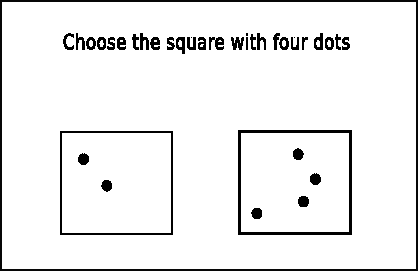
\includegraphics[draft,width=.5\textwidth]{images/stimuluse1}
%\caption{\deleted{Example stimulus from experiment 1. Stimulus consists of two elements (1) the two squares with a number of dots, one of which is the referent of the instruction; (2) the text of the instruction that identifies the target with a referring expression.}}
%\label{stime1}
%\end{figure}
%
%\subsubsection{\deleted{Procedure}}
%\deleted{The experiment was conducted in a small quiet room. On arrival in the room, the participant was told that he or she would be presented with objects on screen, together with an instruction to choose one of them by pressing the appropriate key on the keyboard (which was left cloverleaf for a target on the left, and right cloverleaf for a target on the right). The participant was instructed to respond quickly while avoiding errors.
%There were 4 practice trials. After the practice trials the participant was invited to ask any questions they had about the procedure, and then the experimenter left the cubicle before the experimental blocks began.
%The order in which trials were presented was randomised per participant. Each trial would time out after 60 seconds if the participant did not respond. No feedback was given on correct trials, but there was feedback on error trials in the form of the word ``\textsc{wrong!!}" which flashed on screen. Response time was measured from the appearance of the stimulus on screen until the button-press indicating the participant's choice. The trial sequence was keypress $\rightarrow$ instruction and stimulus $\rightarrow$ keypress.}
%
%\subsection{\deleted{Results}}
%
%\deleted{For the response time analysis 40 erroneous trials were removed, and then the data were trimmed at 2.5 s.d. separately for each participant, removing another 60 cases. In all, 6.3\% of the data were removed.}
%
%\deleted{A linear mixed effects regression model was built of the log response time data. The model had vagueness and subitizability as the fixed effects of main interest, and control terms for quantity and gap size, with random slopes for vagueness over items and for the vagueness x subitizability interaction over subjects.}
%
%\deleted{The main effect of subitizability was significant: subitizable stimuli resulted in faster responses than non-subitizable stimuli ($\beta=-.303, se=.062, t=-4.867, p=.002$). The main effect of vagueness was not significant ($\beta=.017, se=.021, t=.809, p=.435$). However vagueness did exert an interaction effect with subitizability ($\beta=.172, se=.037, t=4.640, p<.01$), such that vagueness increased response times when the analysis was restricted to only subitizable stimuli ($\beta=.103, se=.035, t=2.930, p<.05$). but reduced response times when the analysis was restricted to non-subitizable stimuli ($\beta=-.066, se=.023, t=-2.826, p<.05$). }
%
%\deleted{Error rates were low at 2.5\% overall. A generalized logit mixed model \protect\cite{jaeger2008categorical} was fit to the error data. Fixed effects were vagueness, subitizability and their interaction, with quantity and gap size as control terms. The random effects structure was random slopes for vagueness and random intercepts for item (models with more complex structure did not converge). A large gap led to fewer errors ($\beta=-.976, se=.443, z=-2.201, p<.05$). There was a reliable vagueness x subitizability interaction ($\beta=2.559, se=.880, z=2.906, p <.01$) with the same shape as that for response times (see Fig \protect\ref{fige1}).}
%
%\begin{figure}
%\centering
%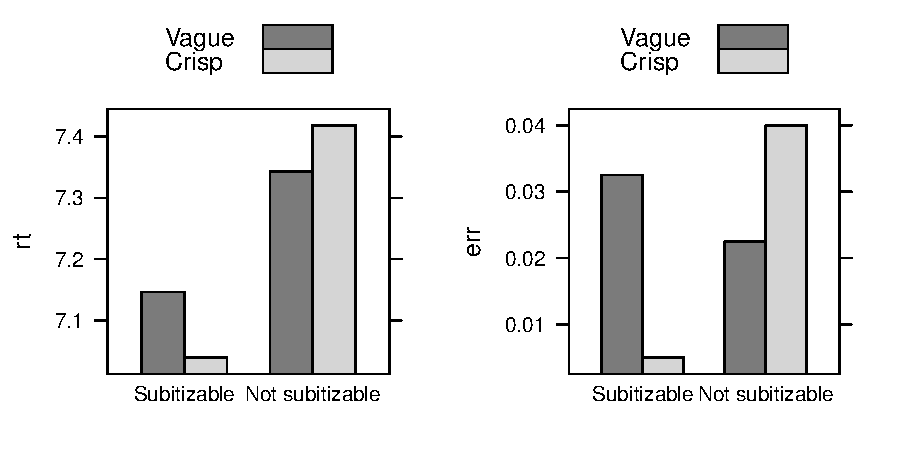
\includegraphics[draft,width=.8\textwidth]{images/resultse1}
%\caption{\deleted{Results for experiment one}\label{fige1}}
%\end{figure}
%
%\subsection{\deleted{Discussion}}
%\deleted{As expected, response times were faster for stimuli that contained a subitizable number of dots. Our main question was whether vagueness would interact with this effect. Response times did not differ reliably according to whether the quantifier was vague or crisp but vagueness did affect response times differently for subitizable and non-subitizable stimuli. When the stimulus contained a subitizable number of dots vagueness slowed responses and led to more errors. When neither square contained a subitizable number of dots, vagueness speeded response times and led to fewer errors.}
%
%% added Feigenson ref - MG
%
%\deleted{A possible explanation of this pattern of results is that when subitizable numbers are present, vagueness hinders the fast automatic system that deals with small numbers, whereas when these specialised routines are not available because there is no subitizable number, vagueness helps participants to identify the right square by allowing them to use estimates of cardinality instead of counting. }
%\deleted{This explanation has some parallels with the two systems for representing number discussed in \protect\citeA{Feigenson2004307}. They write that ``large arrays [\ldots] activate a system for representing sets and comparing their approximate cardinal values'' whereas``small arrays [\ldots] activate a system for representing and tracking numerically distinct individuals, which allows for computations [\ldots] of the number of individuals in the array'' \protect\cite[p.~311]{Feigenson2004307}.}

\section{Experiment Two} 

\subsection{Introduction}
We used a forced choice task to compare choices made in response to vague instructions against choices made in response to crisp instructions. 
The participant was presented with an instruction like ``Choose the square with many dots in the vague conditions", or ``Choose the square with 20 dots in the crisp conditions."
Then two dot arrays were presented in the form of squares containing a number of dots.
The participant was required to identify the square that corresponded with the instruction, by pressing the appropriate key.
Response time and accuracy were recorded for analysis.
\added{Fig \ref{stimuluse2} shows an example stimulus.}

Our main manipulation was of the vagueness of the instruction, with two levels, vague and crisp. Table \ref{instructionse2} shows examples from each condition. 
We also manipulated how discriminable the dot arrays were. One array always contained 25 dots: the other varied between 5, 10, 15, 20, 30, 35, 40, 45 dots. This led to numerical differences of 5, 10, 15, and 20, with lower differences representing less discriminable arrays and larger differences representing more discriminable arrays. There is evidence that when the distance grows between two numbers, they become more easily distinguishable from each other: the \emph{numerical distance effect}, which has been shown for comparing the numerosity of two sets of dots \cite{van123} and for processing Arabic numerals and number words \cite{Dehaene199647}.
Where a number was mentioned in the instruction, it was always in the form of an arabic numeral.

The instructions indicated the larger of the two dot arrays equally often as they indicated the smaller of the dot arrays, so that participants could not systematically choose the larger or smaller array as a response strategy.
There is evidence that when two numbers are presented with the smaller on the left, this left-side presentation facilitates responses indicating the smaller number: the \emph{Spatial-Numerical Association of Response Codes (SNARC)} effect \cite{dehaene1993mental, gevers2006automatic}. We controlled which side the smaller number appeared on to avoid systematic influences of this effect. 

\begin{table}[htbp]
\caption{Table of instructions for the pair (5,25). Experiment Two}
\label{instructionse2}
\begin{tabular}{rl}
\toprule
vagueness&example\\
\midrule
crisp 	& 	Choose the square with 5 dots \\
vague	&	Choose the square with few dots\\
\bottomrule
\end{tabular}
\end{table}

\subsection{Hypotheses}
%We hypothesised that under these conditions: (1) RT will be faster for vague than precise instructions; (2) Vagueness will be more advantageous at smaller gap sizes (i.e., low discriminability) than at large gap sizes (i.e, high discriminability). 

The {\bf cost reduction} hypothesis predicts that responses will be faster and more accurate for the vague conditions than for the crisp condition because the vague conditions impose a lower cognitive load than the crisp conditions.  The {\bf instruction format} hypothesis predicts that, for non-subitisable numbers, responses will be faster and more accurate in the verbal conditions than in the numerical ones because numbers are harder to process than verbal references to quantities. There is abundant evidence (e.g., \protect\cite{trick1994small}) that very small (i.e., \emph{subitizable}) quantities are recognised and processed by a distinct psychological mechanism that differs from that used to process larger quantities. We performed a pilot experiment in which we were able to confirm this finding in the experimental settings on which we are focussing in this paper \cite{our-earlier-paper}. In particular, we found that, when participants were confronted with an array of two boxes, instructions of the form ``Choose the square with $n$ dots" led to consistently lower Response Times than instructions of the form ``Choose the square with many/few dots" when $2 \leq n \leq 5$. The converse was true for $n>5$. % KvD: Can you check this addition about subitisable numbers, Matt? I'm not sure this stuff has found its right place in the paper yet. Where it is at the moment, it seems to break the story. Is it better after all to make this Experiment 1 (announced as a replication)?
The {\bf selection algorithm} account predicts that responses will be faster and more accurate in the comparison conditions than in the matching conditions because it is easier to carry out comparison than matching. Thus all three accounts predict a main effect advantage of vagueness, but for different reasons.

Regardless of which of the above hypotheses one adopts, one would predict that responses will be faster and more accurate when the numerical distance between the dot arrays is greater than when it is smaller because greater distances result in more easily discriminable arrays. Thus all three accounts predict a main effect of numerical distance, or gap size. For the same reason, one would predict that any advantage for the vague instructions should be smaller than when the arrays are least discriminable. This constitutes a prediction for an interaction between vagueness and numerical distance. % I've combined the old points (2) and (3) and removed the numbering. Maybe you can polish this further, finding a better place for these observations?

% KvD I've tentatively deleted the following. I think it's probably superfluous.
%The present experiment will demonstrate an advantage for our vague conditions, but not that the advantage is due to the vagueness of the instruction, because the vague conditions were also (a) verbal not numeric and (b) answerable with a comparison strategy not a matching strategy.  Our subsequent experiments will discriminate between the alternative accounts.

% KvD I'm tentatively starting with a general explanation of the methodology of this group of experiments.

{\bf General.} All our experiments shared essentially the same methodology: Participants aged between ..., self-reported fluent speakers of English, were recruited by .... and were paid 10 ponds for participating. All had normal, or corrected-to-normal vision. A MacBook ... Stimuli were created ... In all except the last experiment (Experiment 5), items were presented as follows: (...) (IF WE DO ADD THIS GENERAL DESCRIPTION THEN REMOVE THE RELEVANT INFO FROM THE DESCRIPTION OF EACH OF THE INDIVIDUAL EXPERIMENTS.)

\subsection{Method}
%\subsubsection{Participants}
Twenty participants were recruited by mailing list and paid ten pounds for participating. Participants were aged between 18 and 45, with a median age of 26. All participants self-reported fluency in English, and had normal, or corrected-to-normal vision.

%\subsubsection{Apparatus}
A MacBook Pro laptop computer with a 13 inch screen presented the stimuli to the participants. Stimuli were created and presented using the language GNU Octave \cite{eaton:2002} and the Psychophysics Toolbox extensions \cite{ptbx1, ptbx2}.

%\subsubsection{\deleted{Design}}
\deleted{We presented participants with 256 trials, arranged in 4 blocks of 64 trials each. }


\deleted{It was always the case that two squares appeared on screen. One of these always contained 25 dots, and the other contained a number of dots that varied, and which was always the target. }

\deleted{We can use the notation $pair_{(p)}(n,25)$ to represent a pair. The pairs were: $pair_{(1)}(5,25)$; $pair_{(2)}(10,25)$; $pair_{(3)}(15,25)$; $pair_{(4)}(20,25)$; $pair_{(5)}(30,25)$; $pair_{(6)}(35,25)$; $pair_{(7)}(40,25)$; $pair_{(8)}(45,25)$.}
%
\deleted{We manipulated two independent variables: gap size, with four levels (gap size = 5, 10, 15, or 20), and vagueness, with two levels (crisp and vague). }
\deleted{We had to control another two variables: target size (whether the referring expression indicated the larger number of dots or the smaller number of dots); and target side (for a given level of target size, whether the target appeared on the left or the right). }
\deleted{We measured, as our dependent variables, response time and response accuracy.}
%
\deleted{Our manipulation on gap size divided the items into four groups, one for each gap size. Items with gap size 5 were: $pair_{(4)}(20,25)$; and $pair_{(5)}(30,25)$; items with gap size 10 were: $pair_{(3)}(15,25)$; and $pair_{(6)}(35,25)$; items with gap size 15 were $pair_{(2)}(10,25)$ and $pair_{(7)}(40,25)$; and items with gap size 20 were $pair_{(1)}(5,25)$ and $pair_{(8)}(45,25)$.}
%
\deleted{Our manipulation on vagueness meant generating vague and crisp versions of each referring expression. Each pair was presented 8 times with a vague expression of quantity, and 8 times with a crisp expression of quantity. Taking $pair_{(1)}(5,25)$ as an example, the crisp referring expression was ``Choose the square with 5 dots'', and the vague referring expression was ``Choose the square with few dots''.
%
We needed to control which side the target was presented on. Each pair was presented equally often with with the target on the left, as with the target on the right.
%
We also needed to control whether the target was the smaller or larger number. The items with numbers less than 25 (pairs 1 to 4) formed a group with the smaller number as target and the other items (pairs 5 to 8) formed a balancing group with the larger number as the target number.}


%\subsubsection{\deleted{Stimuli}}

\deleted{Each stimulus consisted of two elements (a) the text of the referring expression indicating the target; (b) two squares containing dots. }
\deleted{Where a number was mentioned in the instruction, it was always in the form of an arabic numeral (e.g., 1,2). }
\deleted{This contrasts with experiment one, where numbers were given in natural language form.}
\deleted{The position of the dots was randomised per-trial.}
\deleted{Fig (\ref{stimuluse2}) gives an example stimulus.}

\begin{figure}[tbp]
\fitfigure{images/stimuluse2}
\caption{An example stimulus from Experiment Two. First the referring expression was presented (left panel). Then after a keypress, and a fixation cross (not pictured) the squares and dots were presented without repetition of the referring expression (right panel)}
\label{stimuluse2}
\end{figure}

%\subsubsection{Procedure}

The experiment was conducted in a quiet room. On arrival in the room, the participant was told that he or she would be presented with an instruction to choose one of two squares by reference to how many dots it contained. Participants were required to press the space key after reading the instruction. Then there was a central fixation cross for 1000 ms, and a blank screen for 500 ms, followed by the squares and dots (without repetition of the referring expression).  The position of the dots was randomised per-trial. Response time was measured as the latency between the presentation of the dots and squares, and the keypress identifying the decision; in this way, the Response Times can be separated from readings times, which is important since we are only interested in the latter. % KvD OK?

The display would stay on screen until the participant responded (there was no timing-out). Participants were asked to respond quickly while avoiding errors. There were 8 practice trials, after which the participant was invited to ask any questions about procedure. After answering these the experimenter left the cubicle for the duration of the experiment. The order in which trials were presented was randomised per-participant. There were 256 trials, presented in 4 blocks of 64 trials each, between which the participant could rest. No feedback was given on correct trials, but there was feedback on error trials in the form of the word ``\textsc{wrong!!}'' which flashed on screen.

\subsection{Results}

A response was counted as erroneous if the square with the wrong number of dots was chosen (when the instruction contained a number); if the square with the larger number of dots was selected (when the instruction was ``Choose the square with few dots"); or if the square with the smaller number of dots was selected (when the instruction was ``Choose the square with many dots".) % KvD Is this addition defining "erroneous" OK?
RTs for trials with erroneous responses were discarded, leading to the loss of 354 trials from 5120, representing 6.9\% of the trials. The correct response RTs were trimmed at 2.5 standard deviations for each subject, leading to the loss of 160 trials, 3.4\% of the correct responses. Means for response times and error rates are given in Fig. (\ref{resultse2}).
A linear mixed model of RT was built using as independent variables vagueness and gap size and their interaction, with random slopes for vagueness and gap size over participants. Vagueness was sum coded: vague $= -.5$, crisp $= .5$; gap size was Helmert coded. Helmert contrasts compare each level against the mean of the previous levels. Level one of this contrast is gap size 5 compared with gap size 10; level two is the mean of gap size 5 and gap size 10 versus gap size 15; and level three is the mean of gap sizes 5, 10 and 15 versus gap size 20. 
$p$ values were calculated using the R package \emph{lmerTest} \cite{lmerTest}.

RTs were faster for vague instructions ($\beta=.109, se=.022, t=4.9, p<.001$). 
%
RT grew faster as gap size increased: level one $(\beta=-.116, se=.012, t=-9.3, p<.05)$, level 2 ($\beta=-.103, se=.009, t=-11.1, p<.001$) and level three ($\beta=-.082, se=.007, t=-11.0, p<.05$). Since discriminability of the dot arrays is easier for larger gap sizes, discriminability probably underlies this effect. Gap size and vagueness interacted significantly for larger gap sizes when modelling RT. % KvD Is it worth saying how they interacted?
The interactions at the different levels of gap size were: level one: ($\beta=.001, se=.016, t=.03, p=.974$); level two ($\beta=-.039, se=.009, t=-4.460, p<.001$); level three ($\beta=-.043, se=.006,t=-7.0, p<.001$). In the crisp conditions RTs started out much slower than in the vague conditions, at the smallest gap size, but the two conditions converged to very fast times at the largest gap size. There were diminishing returns for vagueness as gap size increased. 

\label{accann}
Error rate data were analysed using a generalized logit mixed model \cite{jaeger2008categorical}, with vagueness and gap size and their interaction as independent variables, and with random slopes for vagueness and gap size over participants. 
%
The effect of vagueness on error rates approached significance, with the vague instructions leading to fewer errors ($\beta=.307, se=.173, t=1.8, p=.077$).
%
Error rates decreased as gap size increased: level one ($\beta=-.585, se=.092, ,z=-6.4, p<.001$), level 2 ($\beta=-.434, z=-5.3,p<.001$) and level three ($\beta=-.250,z=-4.1, p<.001$). 
%
Error rates were greater in the crisp conditions than the vague conditions when gap size was small, and this difference diminished with increasing gap size until it reversed at the biggest gap size.
\begin{figure}[htbp]
\fitfigure{images/plotMeansBoth.pdf}
\caption{Experiment Two results. }
\label{resultse2}
\end{figure}

\subsection{Discussion}

The experiment provided support for hypothesis (1), that responses would be faster and more accurate for the vague instruction conditions than for the crisp instruction conditions. 
We also found that responses grew faster and more accurate as the numerical distance between the dot arrays grew larger, in line with hypothesis (2).
The experiment also provided support for hypothesis (3) that vagueness would be more advantageous at smaller than at larger gap sizes.  
The findings of Experiment Two might be summarised thus: vague instructions are easier to process than crisp instructions, and returns for vagueness diminish as the stimuli become more easily discriminable. 

The cost reduction hypothesis explains the vagueness advantage by claiming that the vague referring expressions place less cognitive load on the comprehender than the crisp referring expressions. It explains the diminishing returns for vagueness in more-discriminable stimuli by claiming that load is low in both conditions for the easily-discriminable stimuli, and that therefore there is no extra benefit to be had from vagueness in the easily-discriminable stimuli. 

The instruction format hypothesis explains the main effect advantage for the vague instructions by observing that the vague instructions used verbal quantifiers whereas the crisp conditions used numerical quantifiers. Under this account it is avoiding numbers that explains the vagueness advantage main effect. The main effect of numerical distance is explained by assuming that larger distances result in more easily discriminable arrays. The vagueness x numerical distance interaction can be explained by assuming that the numerical quantifiers make the task particularly challenging when the stimuli are less discriminable.

The selection algorithm account explains the main effect advantage of the vague conditions as due to the vague conditions allowing a comparison strategy rather than a matching strategy in the crisp conditions. The main effect of numerical distance is explained by claiming that comparison is easier for more discriminable arrays. The diminishing returns for vagueness as numerical distance grows are explained by claiming that the advantage of being able to use comparison is greater for less discriminable arrays than for more discriminable arrays.

%A possible explanation for the pattern of results is cast in terms of the precision of an estimate of quantity that is required to carry out the task. For example, in the display pair$_{(1)}(5, 25)$, with a large gap size, vague instructions (\emph{many}, \emph{few}) might be able to  be carried out by a visual comparison that identifies one square as more numerous than the other. Precise instructions (to identify the square with 5 dots) might be able to be carried accurately out with an estimate with a fairly large error of 19. In the display pair$_{(8)}(20, 25)$, which has a small gap size, vague instructions might be able to be be carried out with a visual comparison that identifies one square as more numerous than the other. Precise instructions might require an estimate with a maximum error of 4 in this case. The pattern of results can be explained if we assume that the degree to which an estimate with error 4 is harder than an estimate with error 19 is greater than the degree to which a visual comparison between 20 and 25 is harder than a visual comparison between 5 and 25.

%\item An account that we will dub the \emph{instruction format hypothesis}, or the number / no-number account, explains the vagueness advantage by placing importance on the observation that the vague conditions did not mention a numeral whereas the crisp conditions did. This could make the difference between a task that taps numerical processing, and one that taps magnitude judgements. The diminishing returns for vagueness can be explained by assuming that the numerical task is particularly challenging when the stimuli are less-discriminable, whereas the magnitude judgement is relatively less difficult in the less-discriminable trials. 

%\item \citeA{Rayna:1989lr} can account for the pattern in a framework they called the \emph{hierarchy of gist}. They proposed that reasoners encode representations at different levels of precision, and that these representations can be ordered with respect to precision, forming a hierarchy of gist. They further claimed that reasoning operated at the lowest level in this hierarchy that would allow one to accomplish the assigned task. Among the levels of this hierarchy are  (1) ratio representations at the top, which encode numerical information exactly; (2) ordinal representations that capture relative magnitude but do not encode numerical differences, i.e., they establish a rank ordering of quantities by magnitude, e.g., \emph{large}, \emph{larger}, \emph{largest}; (3) nominal or categorical representations that capture only the presence of absence of quantity e.g., \emph{some lives}; \emph{no lives}. \citeA{brainerd1994development} presented evidence that children spontaneously encode relative numerosity, at the ordinal level of the hierarchy mentioned above, when they are presented with stimuli that vary in numerosity. The hierarchy of gist offers an explanation of our vagueness advantage in experiment two that is independent of vagueness in the \citeA{keefe1996vagueness} sense. In experiment two, the participants were presented with the instruction for the trial first, and then with the squares and dots. This was done in order to try to separate the processes involved in processing the instruction from those involved in processing the stimuli. A consequence of this serial presentation though is that participants can infer from the instruction which level of representation is the minimum level necessary to carry out the impending task successfully. We do not suggest that this takes the form of a conscious deliberation -- rather it might be apprehended spontaneously in the same way that the children in \citeA{brainerd1994development} did without conscious deliberation. For example, it follows naturally from the instruction \emph{Please choose the square with fewest dots} that an ordinal representation will be necessary and sufficient for the purposes of the current trial: similarly it follows naturally from the instruction \emph{Please choose the square with 34 dots} that a higher level of the hierarchy will be necessary and sufficient for the purposes of this trial - the ratio level that encodes numerosity exactly. We found a response time advantage in experiment two for instructions that used the quantifiers \emph{many} and \emph{few}, when compared with times for quantifiers like \emph{15} and \emph{45}. In the terms of \citeA{Rayna:1989lr}, this can be explained as an advantage for the sufficiency of a lower level of representation -- without reference to vagueness.
%
%\item The \emph{two-systems account} of decision making \cite<e.g.,>{sloman2007two} can offer an explanation of the pattern. Dual process models of decision making propose two systems of processing: the quick and affective System 1 and the deliberative and rule-based System 2. This two-systems account can explain our finding of diminishing returns for vagueness in experiment 2. When the gap size is small, participants use System 2 (slow, deliberative) for the precise instructions. When the gap size is large, they take a shortcut for the crisp conditions and merely establish which square is more (or less) numerous, using System 1 (quick, heuristic). In the vague conditions, they use the heuristic system whether the gap size is small or large. This account explains the diminishing returns for vagueness that we observed in terms of a change of strategy in the baseline precise conditions as the gap size grew larger.
%\end{seriate}

%The potential for vagueness in the vague conditions can be said to have been unrealised in Experiment Two. The vague instructions were  \emph{choose the square with many dots} and \emph{choose the square with few dots}. \emph{Many} and \emph{few} have the potential for vagueness defined as the existence of borderline cases. Given a square with 15 dots, and asked the question `are there many dots in the square?', we can imagine that some people would be unsure (contrast this with the questions `are there fewer than 20 dots in the square?' to which there is no room for uncertainty). However, this potential for vagueness may be unrealised in the context of a choice between two squares. Given two squares, one with 20 dots, and another with 25 dots, and asked to `choose the square with few dots', it seems that no one could be unsure which square is the intended target. If there is no room for uncertainty, then the potential for \emph{many} and \emph{few} to be vague can be said to be unrealised. 

\section{Experiment Three}

\subsection{Introduction}

The main result from experiment two was that responses were faster and more accurate for vague instructions than for crisp instructions. This finding can be interpreted in line with three different hypotheses.%: the cost reduction hypothesis, the instruction format account, and the selection algorithm account. 
In experiment three we set out to distinguish between the cost reduction hypothesis and the instruction format account, leaving the selection algorithm account for experiments four and five. Contrast an expression from the vague condition: `the square with few dots' with an expression from the crisp condition: `the square with 15 dots'. One difference is that `few' is vague (or at least has the potential for vagueness) and `15' is crisp. Another difference is that `few' is a linguistic, or verbal quantifier while `15' is a numerical quantifier, in the sense that a number is mentioned explicitly. Since these two differences were confounded in Experiment Two, the vagueness advantage finding is vulnerable to an alternative interpretation, that what we saw as a vagueness advantage was in contrast an advantage for the linguistic or verbal form of the quantifier. In the present experiment three we pitted these alternative interpretations against each other in a factual design. 

In Experiment Two, the participants chose one of two squares. The `vague' quantifiers (e.g., `few') uniquely identified one square. Recall our definition of vague  -- ``a word is precise if it describes a well-defined set of objects. By contrast, a word is vague if it is not precise''.  In the first experiment, the quantifiers in the vague conditions did not really meet this definition. This is because there were no borderline cases of the referent that could make the referent set `not well-defined'. Experiment three used three squares so that the vague quantifiers always had more than one possible referent. To enhance the potential for the vague quantifiers to have true vagueness in Experiment Three, we also used indefinite articles in the vague instructions. Thus, instead of the instruction \emph{Choose the square with few dots}, we used \emph{Choose a square with few dots}.

In experiment three, an item was a referring expression followed by a trio of numbers, representing the number of squares in the left, middle, and right squares. We used four different triples of numbers: (6,15,24); (16,25,34); (26,35,44); (36,45,54). Each triple had the following properties: it comprised three squares (instead of two as in Experiment Two); the central number was always presented in the middle of the three; there were two flanking numbers where one was smaller than the central number and one was bigger. 

There was a numerical and a verbal version of each of the vague and crisp referring expressions. See Table \ref{instructionseB} for examples.
The vague numerical condition's referring expression was ``Choose a square with about 10 dots''. None of the squares displayed contained 10 dots. %10 is slightly closer to 6 than to 15. Therefore the best referent for this referring expression was the square with 6 dots;  the borderline response was the square with 15 dots; and the poorest referent was the square with 24 dots. 
% KvD: tentatively removed the above.
%
% KvD: In what follows, I've made a number of fairly trivial replacements and reorderings. Please check!
The {\em crisp numerical} conditions's referring expression was ``Choose the square with 6 dots'' on half the presentations in that condition and ``Choose the square with 24 dots'' on the other half. One square did contain the exact number mentioned.  In the {\em crisp verbal} condition, we used the referring expression ``Choose a square with fewer than $20$ (more than $10$) dots".  The {\em vague numerical} condition's referring expression was ``Choose the square with far fewer than $20$ dots'' on half of presentations, making the squares with 6 and $15$ dots possible referents; iin the other case, the referring expression was ``Choose the square with far more than $10$ dots'', which made $15$ and $24$ possible referents.The {\em vague verbal} condition's referring expression was ``Choose a square with few dots'' on half of the presentations, and ``Choose a square with many dots'' on the other half. For this condition, the best referent was the square with 6 dots for `few' and 24 dots for `many'; the borderline case was the square with 15 dots; and the remaining square was the poorest referent. 
% KvD: OK, Matt? This needs checking once again.
%
% An indication that the manipulation of vagueness was successful is that participants chose the borderline case square on 16\% of trials.
% KvD This last sentence needs to be reformulated, talking about {6,15} both.


\begin{table}[htbp]
\caption{Table of instructions arranged by condition for the triple (6,15,24). Experiment Three}
\label{instructionseB}
\begin{tabular}{rlll}
\toprule
vagueness&instruction format&selection task&example\\
\midrule
crisp 	& 	numeric	& matching	&Choose the square with 6 dots \\
vague	&	numeric 	& matching	&Choose a square with about 10 dots\\
crisp		&	verbal	& comparison	&Choose the square with the fewest dots\\
vague	&	verbal	& comparison	&Choose a square with few dots\\
\bottomrule
\end{tabular}
\end{table}

\subsection{Hypotheses}
The instruction format account predicts a main effect of instruction format such that the numeric instruction conditions will attract longer response times, but has no prediction of any vagueness effects or interaction effects with vagueness.  

The selection task account predicts the same main effect but treats it as an effect of the task mandated by the instruction, with the matching task conditions predicted to take longer than the comparison task conditions.  

The cost reduction account predicts that there will be a main effect of vagueness such that the vague instruction conditions attract faster responses than the crisp instruction conditions. The cost reduction account also predicts an interaction with the instruction format (or selection task) variable: at each level of instruction format (or selection task) the vague condition should attract faster responses than the crisp condition.

\subsection{Method}

Thirty participants were recruited and paid in the same way as Experiment Two. They were aged between 18 and 45 with a median age of 28. All participants self-reported fluency in English, and had normal, or corrected-to-normal vision.

The same apparatus was used as for Experiment Two.

We presented participants with 256 trials, arranged in 4 blocks each with 64 trials. Each triple was presented in each condition 16 times. 8 of these identified the larger number, and 8 the smaller. We manipulated two independent variables: vagueness with two levels (vague and crisp); and instruction format with two levels (numeric, verbal). In this experiment the selection task variable mapped onto the instruction format variable: the numeric instruction conditions both mandated a matching selection task and the verbal instruction conditions both mandated a comparison task. This yielded four conditions (vague numeric; vague verbal; crisp numeric; crisp verbal). Each condition had a different referring expression, as follows, using the triple $(6,15,24)$ as an example: Choose a square with about 10 dots; Choose a square with few dots; Choose the square with 6 dots; Choose the square with the fewest dots. We measured two dependent variables: response time; and the probability of a participant choosing the borderline case.

Fig (\ref{stimuluse3}) gives an example stimulus. First, the referring expression that constituted the instruction for that trial was displayed. The participant then pressed a key to indicate that he or she had read the instruction. After 1 second,  the squares and dots were presented, while preserving the text of the referring expression. The position of the dots in the squares was randomised per-trial.

\begin{figure}[tbp]
\centering
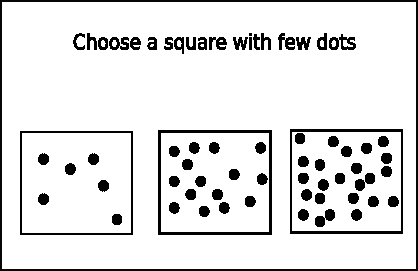
\includegraphics[width=.4\textwidth]{images/stimuluse3}
\caption{An example stimulus from Experiment Three}
\label{stimuluse3}
\end{figure}

The experiment was conducted in a small quiet room.
On arrival in the cubicle, the participant was told that he or she would be presented with objects on screen and required to choose one in response to an instruction on screen, by pressing the button corresponding with the object. There were 5 practice trials. After the practice trials the experimenter left the room. There were 4 blocks of 64 trials each. In between blocks the participant had the opportunity to rest before continuing. The response time dependent variable was measured from the presentation of the squares and dots, until the keypress indicating the participant's choice. The trial would timeout after 60 seconds if there was no response. The dependent variable measuring whether the participant chose the borderline case was also recorded at this time. In this experiment, no feedback was given. This was because, in the vague conditions, we did not regard any response as `correct' or `incorrect', but instead as `borderline response', or `not borderline response', and we did not want to draw participants' attention to this distinction explicitly. We simply recorded whether the participant chose the borderline case or not, and how long it took the participant to respond.

\subsection{Results}

This time around, no responses were treated as erroneous, because errors were essentially undefined for the vague instructions (e.g., `about ten'). It was noted whether participants chose the borderline square. 
%
The RTs were trimmed at 2.5 standard deviations for each subject, leading to the loss of 236 trials, 3.1\% of the data. Means for response times and error rates are given in Fig. (\ref{resultse3}).

A linear mixed model was constructed for the response times, with selection task (or instruction format), vagueness, and item and their interactions as independent variables, and random slopes over participant for task and vagueness (and their interaction) and for item. Task and vagueness were sum coded and item was centred. There was a significant effect of task with numerical conditions attracting longer responses than the verbal conditions ($\beta=.37, se=.07, t=5.1, p<.001$). The effect of vagueness was to slow responses down  ($\beta=.058, se=.013, t=4.8, p<.001$). There was an interaction effect between vagueness and task, such that the disadvantage for vagueness was greater in the numerical than in the verbal instruction conditions.  There were differences in response time as a function of item ($\beta=.06, se=.008, t=7.0, p<.001$) but there was no clear trend across items.

Participant grand mean percentage of borderline selections was $16.6\%$. A generalized linear mixed model \cite{jaeger2008categorical} was fit to the data for selection of the borderline response, with task, vagueness and item as fixed effects, and with random slopes for task and vagueness and item over participants.  Participants were significantly more likely to choose the borderline option for vague instructions than for precise instructions (21.9\% vs 11.3\%, $\beta=.79, se=.25, z=3.2, p<.01$). Participants were significantly more likely to choose the borderline square when the instruction used the numerical format rather than the verbal format (30.1\% vs 3.0\%, $\beta=3.57, se=.26, z=13.6, p<.001$). 

\begin{figure}[htbp]
\centering
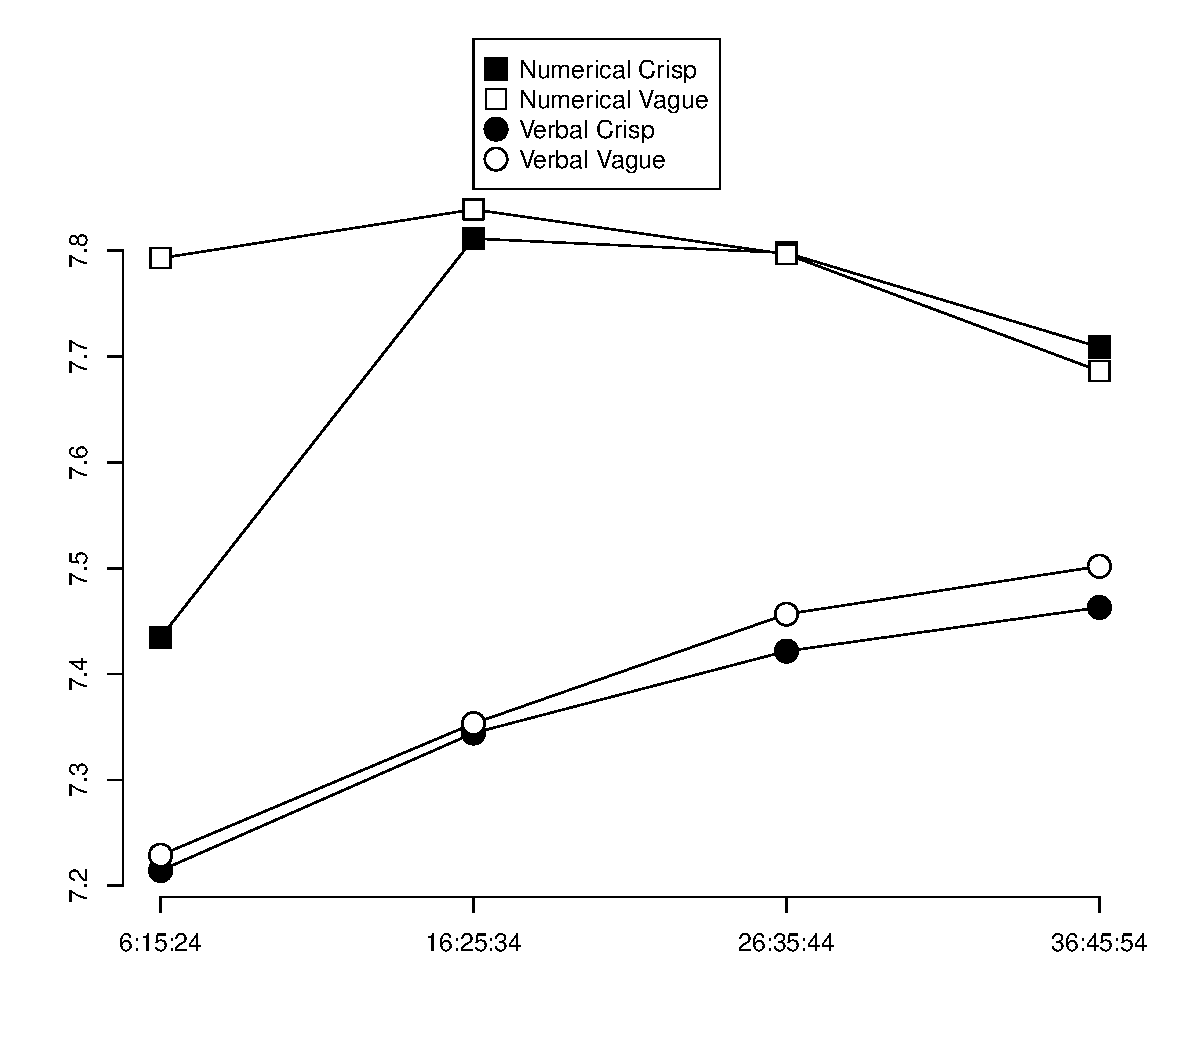
\includegraphics[width=.65\textwidth]{images/resultse3.pdf}
\caption{Results for Experiment Three}
\label{resultse3}
\end{figure}

\subsection{Discussion}

This experiment tested to see whether when borderline cases are present, vague instructions would speed responses as they did in Experiment Two when there were no borderline squares. We actually found a \emph{disadvantage} of vague instructions: vague instructions slowed people down by 112 ms on average. We also found that the effect of instruction format was significant, with numerical format slowing responses by 689 ms on average. The disadvantage of numerical format overwhelms the contribution of vagueness. The verbal vague condition was still responded to faster than the numerical crisp condition, so the pattern from Experiment Two is reproduced, but in the light of the evidence from Experiment Three in the presence of borderline cases, the advantage that was ascribed to vagueness before now looks more like either an advantage of verbal instruction format, or alternatively as an advantage of the comparison task, according to the selection task account.

% KvD: I've tentatively added the following:
Having effectively separated the {\bf cost reduction} hypothesis from the {\bf instruction format} hypothesis, it is important to observe that, in Experiment 3, instruction format went hand in hand with {\bf selection algorithm}: as shown by the Table of instructions \ref{instructionseB}, the instructions that used a verbal instruction format allowed a comparison algorithm, whereas the instructions that used a numeric format allowed on a matching algorithm. Therefore, our results so far permit the interpretation that what made the instructions in the verbal condition fast is not the fact that they were worded verbally, but that they allowed participants to use a comparison algorithm (which is known to be faster than matching). % KvD I assume we need to say more about this, citing some appropriate papers to support this idea.

In the next two experiments we pitted the comparison and matching selection tasks against each other while controlling vagueness and instruction format. In Experiment Four we would restrict all the instructions to numeric quantifiers while factorially manipulating vagueness and the comparison / matching selection tasks. In Experiment Five we would ensure that all instructions used verbal quantifiers, while also factorially manipulating vagueness and the comparison / matching selection tasks. This allows us to distinguish between the predictions of the selection task account and the instruction format account. 

\section{Experiment Four}

\subsection{Introduction}

The main aim of experiment four was to see whether vagueness would exert beneficial effects when all conditions used numerals in the instructions, and when there were vague and crisp versions of the instructions for both comparison and matching strategies. The main changes from experiment three were that the selection task was explicitly controlled, and that all conditions were constrained to mention a number. We used the same stimuli as in experiment three. Table \ref{Instructions for e4} shows the instructions. % KvD I think we should motivate our choice of materials (especially "far ..er")

\begin{table}[htbp]
\centering
\caption{Experiment Four: Instructions, assuming $6,15,24$ dots as the Item, and showing \emph{fewer} instead of \emph{more}}
\label{Instructions for e4}
\begin{tabular}{llll}
\hline
vagueness&instruction format&selection task&instruction\\
\hline
crisp & numeric&matching & Choose a square with 6 dots \\ 
crisp & numeric&comparison & Choose a square with fewer than 20 dots \\
vague & numeric&matching & Choose a square with about 10 dots \\ 
vague & numeric&comparison & Choose a square with far fewer than 20 dots \\ 
\hline
\end{tabular}
\end{table}%


\subsection{Hypotheses}
% (1) Vague instructions are easier for the reader than crisp alternatives (main effect of vagueness)
%(2) Comparison is easier for the reader than matching (main effect of selection)
%(3) Effects of vagueness are different depending on whether selection is matching or comparison (interaction effect selection x vagueness).

The instruction format account predicts no differences between the conditions, since all conditions used numeric quantifiers.

The selection task account predicts a main effect of selection task such that the comparison conditions would attract faster responses than the matching conditions.

The cost reduction account predicts that there will be a main effect of vagueness such that the vague instruction conditions attract faster responses than the crisp instruction conditions and particularly that at each level of selection task the vague condition should attract faster responses than the crisp condition.


\subsection{Method}

38 volunteers were recruited via internal messaging at University of Aberdeen, with self-reported fluency in English. They were paid ten pounds each for participating.
The apparatus was the same as Experiment Two.
The design was a 2 x 2 factorial manipulation of vagueness and selection task (see Table \ref{Instructions for e4}).
Each stimulus was an instruction followed by a triple of dots.
First a referring expression instruction was presented. Participants pressed a key to dismiss the instruction and proceed to the squares with dots in them.

\subsection{Results}
A linear mixed effects regression model was built for log response times. The structure of the model was as follows: fixed effects were vagueness, selection task (both sum coded) and centred item and their interactions: random effects were vagueness, selection task, and item (but not their interactions - the model failed to converge when these interactions were included). The means are plotted in Figure \ref{resultse4}.

The results showed that vagueness was beneficial for comparison but detrimental for matching. There was no significant main effect of vagueness ($\beta =.003, se=.014, t=.202, p=.841$). There was a main effect of task type, with the comparison task speeding responses compared to the matching task ($\beta=-.165, se=.027, t=-6.218, p<.001$). Vagueness exerted effects in different directions for the comparison task and for the matching task. Separate analyses were conducted at each level of the selection task to see whether within each task type there were significant effects of vagueness. There were: in the comparison task vagueness significantly speeded response times compared with crisp controls ($\beta=-.07, se=.02, t=3.52, p<.01$). In the matching task vagueness significantly slowed response times compared with crisp controls ($\beta=-.07, se=.02, t=-2.89, p<.05$).

None of the accounts set out in the Hypotheses section emerge well from the results. The instruction format account wrongly predicts no differences between the conditions. The selection task correctly predicted the main effect of selection task, but has no coverage of the interaction with vagueness. The cost reduction account is wrong to predict main effect advantages for vagueness, and wrong to predict that vagueness should be beneficial at each level of the selection task: however vagueness was advantageous in the comparison task.


\begin{figure}[htbp]
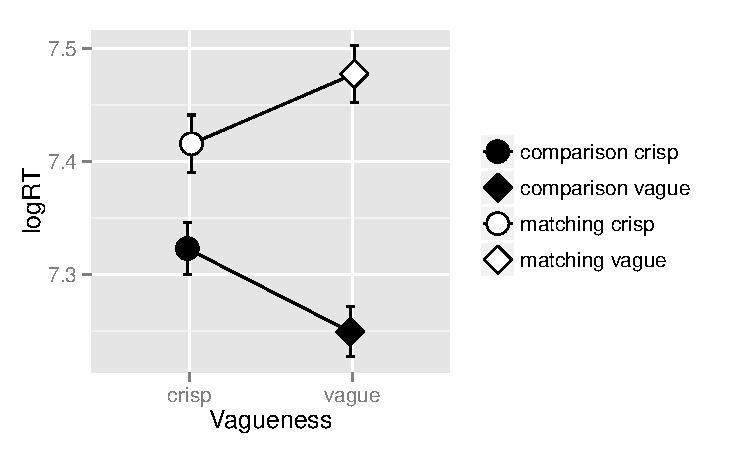
\includegraphics[width=.5\textwidth]{images/resultse4.pdf}
\caption{Results for Experiment Four}
\label{resultse4}
\end{figure}

\section{Experiment Five}
\subsection{Introduction}
This experiment investigated response times for instructions that did not use a number. 
We manipulated vagueness and the selection task (comparison and matching). 
In order to implement the experiment without mentioning numbers,  we used a prime to visually show the numbers of dots that we wanted to refer to as {\em the target} in the instructions. 
\added{This presentation of a prime before the main trial shares some features with Experiment 2 in \protect \citeA{Izard20081221}, although in that experiment participants were told the numerosity of the prime - called an \emph{inducer} in that paper - in our experiment we did not tell participants the numerosity of the prime array.}
An item was thus a combination of a visual prime, a numeric triple, and a referring expression.
The referring expressions were constrained to never mention a numeral, as in Table \ref{Instructions for e5}. 


\begin{table*}[htbp]
\centering
\caption{Experiment Five: Instructions}
\label{Instructions for e5}
\begin{tabular}{lllp{7cm}}
\hline
vagueness&instruction format& selection task&instruction\\
\hline
crisp & verbal&matching & Choose a square with the same number of dots as the target \\ 
crisp & verbal&comparison& Choose a square with fewer dots than the target \\
vague & verbal&matching & Choose a square with about the same number of dots as the target \\ 
vague & verbal&compaison& Choose a square with far fewer dots than the target \\ 
\hline
\end{tabular}
\end{table*}%

\subsection{Hypotheses}
The instruction format account predicts no differences between the conditions, since all conditions used verbal quantifiers.

The selection task account predicts a main effect of selection task such that the comparison conditions would attract faster responses than the matching conditions.

The cost reduction account predicts that there will be a main effect of vagueness such that the vague instruction conditions attract faster responses than the crisp instruction conditions and particularly that at each level of selection task the vague condition should attract faster responses than the crisp condition.

\subsection{Method}

40 volunteers recruited via internal messaging at University of Aberdeen, with self-reported fluency in English. They were paid ten pounds for participating. 
The apparatus was the same as Experiment Two.
The design was a 2 x 2 factorial manipulation of vagueness and selection task.
Each stimulus was a sequence of prime, instruction, and squares.
The procedure for this experiment was different from the others, to accommodate the requirement not to use numbers in the instruction. We had to have a different way to indicate a numerosity in the instruction, which we did by adding a visual `prime', a square that contained the number of dots that we wanted to refer to.

\subsection{Results}
The results showed that vagueness was beneficial for comparison but detrimental for matching (the same as Experiment Four) even when no numbers were allowed in the instructions. Figure \ref{resultse5} shows the means by condition. There was no main effect of vagueness ($\beta=.01, se=.01, t=1.51, p=.14$). There was a main effect of selection, with comparison task instructions leading to faster responses than the matching task instructions ($\beta=-.18, se=.02, t=-10.38, p<.01$). This effect was in the same direction as Experiment Four. Vagueness did  exert different effects depending on the selection task ($\beta=.12, se=.03, t=4.32, p<.05$). Separate analyses were conducted for the comparison task and for the matching task. In the comparison task, vagueness resulted in faster response times ($\beta=-0.08, se=.02, t=4.30, p<.05$). In the matching task vagueness slowed response times ($\beta=.05, se=.01, t=3.72, p<.05$). These results are in the same direction as Experiment Four.

\begin{figure}[htbp]
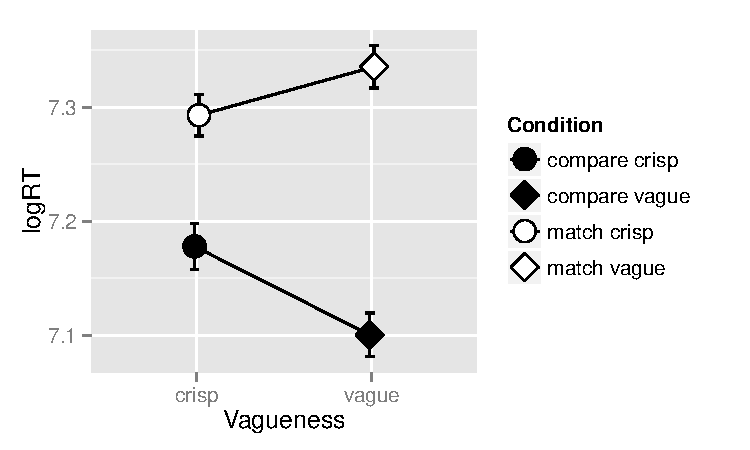
\includegraphics[width=.5\textwidth]{images/resultse5.pdf}
\caption{Results for Experiment Five}
\label{resultse5}
\end{figure}

Again none of the accounts set out in the Hypotheses section emerge well from the results. The instruction format account wrongly predicts no differences between the conditions. The selection task correctly predicted the main effect of selection task, but has no coverage of the interaction with vagueness. The cost reduction account is wrong to predict main effect advantages for vagueness, and wrong to predict that vagueness should be beneficial at each level of the selection task: however vagueness was advantageous in the comparison task.

\subsection{Discussion of experiments 4 and 5}

The main aim of these two experiments was to test whether vagueness confers any cognitive benefits over and above those due to differences in the selection task according to whether the instruction mandates a \emph{comparison} selection task or a \emph{matching} selection task, when number-use is held constant.  The main effect of selection task showed that the assumption that the \emph{comparison} task is easier than the \emph{matching} task is well-founded. In both experiments people were reliably faster at responding in the \emph{comparison} task. 

Vagueness, which was the phenomenon  on which our investigation focussed, did not exert a main effect in response time. However when the comparison and selection tasks were analysed separately, there was small reliable speedup in RT from the crisp to the vague \emph{comparison} tasks, but a small reliable slowdown in RT from the crisp to the vague \emph{matching} tasks. 

\section{General Discussion}

Experiment 2 showed us that responses were faster and more accurate when the instructions were vague than when they were crisp, but the experiment could not distinguish effects of vagueness from those of number-avoidance or selection task: the vague conditions were also in verbal rather than numerical format; and mandated a comparison strategy rather than a matching strategy.  Experiment 3 showed us that number-avoidance in the verbal format instructions is an important factor driving the faster response times in the task, and that vagueness does not have any additional explanatory power in either the verbal format instructions or the numerical format instructions when we generated verbal and numerical versions of both crisp and vague instructions. However the experiment could not distinguish benefits of number-avoidance in the verbal instructions from benefits of the comparison selection task: the verbal instructions also mandated a comparison strategy rather than a matching strategy. In experiments 4 and 5 we manipulated vagueness and the selection task independently of numerical format. We found that there are effects of the selection task mandated by the instruction, with the comparison task instructions attracting faster response times than the matching instructions, and that vagueness exerts benefits when the selection task is \emph{comparison}, but not when the task is \emph{matching}.

The benefits of vagueness in the \emph{comparison} task in experiments 4 and 5 could be explained as differences in the number of valid targets for the expression, as follows. Taking as an example the stimulus with (6,15,24) dots, it could be argued that the vague comparison instruction (e.g., \emph{a square with far fewer than 20 dots}) has one valid target, the square with 6 dots, while the crisp comparison instruction (e.g., \emph{a square with fewer than 20 dots}) has two valid targets, the squares with 6 and 15 dots. In both experiments 4 and 5 we found that people were quicker to identify a square when the instruction only had one valid target. This leads us to speculate that the benefit for vagueness here could be due to the vague expression foregrounding a particular valid target while the crisp expression carries with it the additional task of distinguishing between two alternative valid targets, something we propose to call a ``range-reduction'' benefit.

What is one entitled to conclude? Given that we were able to identify a class of situations -- namely: situations in which a comparison strategy suffices to identify the intended referent -- in which vague expressions led to faster response times than crisp ones, would it be valid to conclude that we have finally discovered an advantage for vagueness that cannot be ascribed to some other factor? We believe the answer to this question is negative. To see why, consider figures \ref{resultse4} and \ref{resultse5}. Both figures depict four conditions, depending on whether the expression was crisp or vague, and depending on whether the referent could be identified using a comparison strategy or not. Two of the resulting four conditions result in an expression that can denote either of two referents; the other two conditions result in an expression that can only denote one referent, with the other possible referent being a marginal candidate at best:

\begin{table}[htbp]
\caption{Vagueness as range reduction}
\begin{center}
\begin{tabular}{lll}
\hline
vagueness & selection task & candidates\\
\hline
crisp & matching & 1 candidate\\
crisp & comparison & 2 candidates\\
vague & matching & 2 candidates\\
vague & comparison & 1 candidate\\
\hline
\end{tabular}
\end{center}
\label{default}
\end{table}

To see why vagueness thus has opposite effects, depending on whether it is used in matching or comparison situations, compare an instruction like `Choose a square with 6 dots' with its vague counterpart `Choose a square with about 10 dots': by adding the word `about', we broaden the range of squares that the expression might be referring to. On the other hand, compare `Choose a square with fewer than 20 dots' with its vague counterpart `Choose a square with far fewer than 20 dots': by adding the word `far', we did not broaden the range of squares denotable by the expression: we narrow it down, because only some of the squares that have fewer dots may have {\em far} fewer dots.

The observation that conditions with 1 candidate lead to shorter response times than conditions with 2 candidates is consistent with the range reduction hypothesis, but not with the idea that vagueness has a beneficial effect. It appears, in other words, that range reduction causes shorter response times, suggesting that shorter response times will only result from a vague expression if this expression leads to range reduction. Once again, it seems, it is not vagueness itself that has advantages but a phenomenon (namely range reduction) that is an automatic concomitant of vagueness in some types of situations.

The findings from our experiments show that when vague expressions are compared with crisp alternatives in our forced choice task, vague expressions appear to yield benefits in some situations, but that the observed benefits may be due to factors other than vagueness itself that the vague forms bring along with them: factors like avoiding numbers; permitting comparison tasks; and range reduction. The picture that is starting to emerge, in other words, is subtle: on the one hand, in the situations that we have been studying -- where cooperative speakers refer to an object (e.g., a square) by means of some quantity associated with the object (e.g., the number of dots contained in the square) -- vagueness is not intrinsically beneficial. On the other hand, vague expressions often have other features that {\em are} beneficial, and these are what give us the incorrect impression that vagueness itself is beneficial. Vagueness may thus have acquired a reputation that it does not deserve. 

A comparison may clarify the logic of the situation. In recent years a number of studies, focussing typically on red wine, have suggested that alcohol, consumed in low doses, may have health benefits. An alternative explanation, however, asserts that it is not the alcohol in the wine that is beneficial, but the antioxidants from grapes. If this alternative explanation is correct then alcohol may not be as beneficial as some of us would have it. % KvD Good hey?

\bibliography{lcn-aug-2014}
\end{document}
